\documentclass[xcolor=dvipsnames]{beamer}
\usepackage{comp2402}
\title{Big O: A Review}
\author{Pat Morin \\ COMP2402/2002}
\date{Carleton University}

\begin{document}

\begin{frame}
  \titlepage
\end{frame}

\begin{frame}
  \frametitle{Big O: Definition} 
   \[ \begin{array}{ll} O(g(n)) = \{ f(n) : &
          \mbox{there exists positive constants $c$ and $n_0$} \\
          & \mbox{such that $f(n) \le cg(n)$ for all $n\ge n_0$} \}\end{array} 
   \]
  \begin{itemize}
  \item<2-> Notice: $O(g(n))$ is a set of functions
   \begin{itemize}
     \item<3-> When we say $f(n)=O(g(n))$ we really mean $f(n)\in O(g(n))$
     \item<4-> E.g., $n^2 + 42n + 7 = O(n^2)$ means:
     \begin{itemize}
       \item<4-> The function $f(n)=n^2 + 42n + 7$ is in the set $O(n^2)$
     \end{itemize}
   \end{itemize}
  \end{itemize}

\end{frame}

\begin{frame}
  \frametitle{$n^2 + 42n + 7 = O(n^2)$}
  \begin{center}
    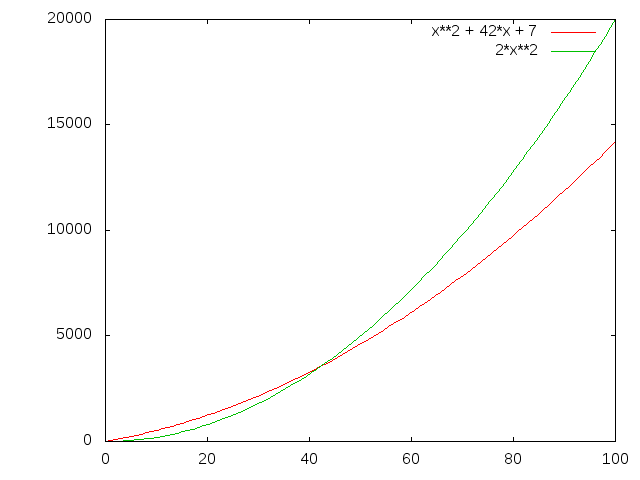
\includegraphics[height=2.5in]{images/graph} \\
    $n^2 + 42n + 7 \le 2 n^2$ for all $n\ge 50$
  \end{center}
\end{frame}

\begin{frame}
  \frametitle{Example}

  \begin{itemize}
    \item Prove $n^2 + 42n + 7 = O(n^2)$
    \item<2-> \[\begin{aligned} 
       n^2 + 42n + 7 
        & \le n^2 + 42n^2 + 7n^2 & \mbox{ for $n\ge 1$} \\ 
        & = 50n^2
      \end{aligned}\]
    \item<3-> So, $n^2 + 42n + 7 \le 50 n^2$ for all $n\ge 1$
    \item<4-> $n^2 + 42n^2 + 7n^2 = O(n^2)$  [ $c=50$, $n_0=1$ ]
  \end{itemize}
\end{frame}

\begin{frame}
  \frametitle{Example}

  \begin{itemize}
    \item Prove $5n\log_2 n + 8n - 200 = O(n\log_2 n)$
    \item<2->[] \[\begin{aligned} 
       5n\log_2 n + 8n - 200
        & \le 5n\log_2 n + 8n \\
        & \le 5n\log_2 n + 8n\log_2 n & \mbox{ for $n\ge 2$ ($\log_2 n \ge 1$)}
            \\
        & \le 13n\log_2 n 
      \end{aligned}\]
    \item<3-> $5n\log_2 n + 8n - 200 \le 13n\log_2 n$ for all $n\ge 2$
    \item<4-> $5n\log_2 n + 8n - 200 = O(n\log_2 n)$ [ $c=13$, $n_0=2$ ]
  \end{itemize}
\end{frame}

\begin{frame}
  \frametitle{Some common relations}

  \begin{itemize}
    \item $O(n^{c_1}) \subset O(n^{c_2})$ for any $c_1 < c_2$
    \item For any constants $a,b,c > 0$,
     \[ O(a) \subset O(\log n) \subset O(n^{b}) \subset O({c}^n) \]
    \item<2-> These make things faster
     \[ 2\log_2 n + 2 = O(\log n) \]
     \[ n + 2 = O(n) \]
     \[ 2n + 15n^{1/2} = O(n) \]
   \item<3-> We can multiply these to learn about other functions,
     \[ O(an) = O(n) \subset O(n\log n) \subset O(n^{1+b}) \subset O(n{c}^n) \]
   \item<4->Examples: $O(n^{1.5}) \subseteq O(n^{1.5}\log n)$
  \end{itemize}
\end{frame}

\begin{frame}
  \frametitle{An indulgence}

  \begin{itemize}
    \item In this course, we see expressions like $O(n-i)$
    \begin{itemize}
      \item Two argument function $g(n,i)=n-i$
      \item \emph{For the purposes of this course}, 
               we will take $O(g(n,i))$ to be
       \[ \begin{array}{ll} O(g(n,i)) = \{ f(n,i) : &
           \mbox{there exists positive constants $c$ and $z$} \\
           & \mbox{such that $f(n,i) \le cg(n,i)$ for all } \\
           & \mbox{arguments such that $f(n,i)>z$} \}\end{array} 
       \]
    \end{itemize}
    \item For example (Lists) valid arguments are $i\in\{0,\ldots,n-1\}$ or (sometimes) $i\in\{0,\ldots,n\}$
  \end{itemize}
\end{frame}

\begin{frame}[fragile]
  \frametitle{Why Use big-O Notation?}
   
  \begin{itemize}
    \item Consider the following (simple) code:
\begin{lstlisting}
  for (int i = 0; i < n; i++) {
    a[i] = i;
  } 
\end{lstlisting}
   \item<2-> The running time is 
   \begin{itemize}
      \item<3-> 1 assignment (\lstinline{int i = 0})
      \item<4-> n+1 comparisons (\lstinline{i < n})
      \item<5-> n increments (\lstinline{i++})
      \item<6-> n array offset calculations (\lstinline{a[i]})
      \item<7-> n indirect assignments (\lstinline{a[i] = i})
      \item<8-> ${}=a + b(n+1) + cn + dn + en$, where $a$, $b$, $c$, $d$, and $e$ are constants that depend on the machine running the code

   \end{itemize}
   \item<9-> Easier just to say $O(n)$ (constant-time) operations
 \end{itemize}

\end{frame}
\end{document}




%\section[Outline]{}
%\frame{\tableofcontents}
%

\section{Convex Hulls}
\frame
{
  \frametitle{Convex Hulls}
  
  \begin{itemize}
    \item Let $P=\{p_0,\ldots,p_{n-1}\}$ be a set of points in the plane
    \item The \emph{convex hull} of $S$
     \begin{itemize}
       \item the smallest convex set that contains $S$.
       \item<2->stretch a rubber band around $S$\only<3->{ and let it go}
    \end{itemize}
    \begin{center}
      \only<1>{\includegraphics{figs/ch-a}} %
      \only<2>{\includegraphics{figs/ch-b}} %
      \only<3->{\includegraphics{figs/ch-c}} %
    \end{center}
  \end{itemize}
}

\frame
{
  \frametitle{Upper and Lower Hulls}
  \begin{itemize}
    \item The \emph{upper hull} of $S$ is a bit simpler
    \begin{itemize}
      \item<2-> get a rope with weights on both ends \only<3->{and throw it over $S$}
    \end{itemize}
    \item<4->For the \emph{lower hull}, use helium-baloons
    \item<5->Convex hull = upper hull + lower hull
  \end{itemize}
    \begin{center}
      \only<1>{\includegraphics{figs/ch-a}} %
      \only<2>{\includegraphics{figs/ch-d}} %
      \only<3>{\includegraphics{figs/ch-e}} %
      \only<4>{\includegraphics{figs/ch-f}} %
      \only<5->{\includegraphics{figs/ch-g}} %
    \end{center}
}

\frame
{
  \frametitle{Summary so far}
  \begin{itemize}
  \item<1-> Input: A set $P$ of $n$ points (unordered)
  \item<2-> Output: A list of the points of $P$ on the convex hull --- in clockwise order
  \item<3-> First compute the upper hull, then the lower hull
  \end{itemize}
  \begin{center}
    \only<1>{\includegraphics{figs/ch-io-a}}%
    \only<2->{\includegraphics{figs/ch-io-b}}%
  \end{center}
}

\frame
{
  \frametitle{Graham's Scan}

  \begin{tabular}{p{3in}p{1.5in}}
    {\vspace{-2in} \begin{itemize}
      \item<1->Invented by Ron Graham in 1973
      \item<2->Sorts the points by $x$-coordinate
      \item<3->Constructs the upper hull incrementally using a stack
    \end{itemize} }
    &
    {\includegraphics[height=2in]{images/graham-12ball} }
  \end{tabular}
}

\frame{
  \frametitle{Graham's Scan}

  \begin{enumerate}
  \item<2->Sort the points by $x$-coordinate
  \item<3->Create a stack $s$ containing $\langle p_0,p_1\rangle$
  \item<4->For $i=3$ to $n$ do
   \begin{itemize}
    \item add $p_i$ to the convex hull of $p_1,\ldots,p_{i-1}$
   \end{itemize}
  \end{enumerate}
  \begin{center}
    \only<1>{\includegraphics{figs/ch-graham-a}}%
    \only<2>{\includegraphics{figs/ch-graham-b}}%
    \only<3>{\includegraphics{figs/ch-graham-c}}%
    \only<4>{\includegraphics{figs/ch-graham-d}}%
    \only<5>{\includegraphics{figs/ch-graham-e}}%
    \only<6>{\includegraphics{figs/ch-graham-f}}%
    \only<7>{\includegraphics{figs/ch-graham-g}}%
    \only<8>{\includegraphics{figs/ch-graham-h}}%
    \only<9>{\includegraphics{figs/ch-graham-i}}%
    \only<10>{\includegraphics{figs/ch-graham-j}}%
    \only<11>{\includegraphics{figs/ch-graham-k}}%
    \only<12>{\includegraphics{figs/ch-graham-l}}%
    \only<13>{\includegraphics{figs/ch-graham-m}}%
    \only<14->{\includegraphics{figs/ch-graham-n}}%
  \end{center}
}

\frame
{
  \frametitle{Adding $p_i$}
  \begin{itemize}
    \item Suppose #s# contains the upper hull of $p_0,\ldots,p_{i-1}$
    \item We want to compute upper hull of $p_0,\ldots,p_{i}$
    \begin{enumerate}
    \item while #s.get(s.size()-2)#, #s.get(s.size()-1)#, and $p_i$ form a left turn
    \begin{itemize}
      \item #s.remove(s.size()-1)# (pop)
    \end{itemize}
    \item  #s.add(#$p_i$#)#
    \end{enumerate}
  \end{itemize}
  \begin{center}
    \only<1>{\includegraphics{figs/ch-graham-e}}%
    \only<2>{\includegraphics{figs/ch-graham-e-a}}%
    \only<3>{\includegraphics{figs/ch-graham-e-b}}%
    \only<4>{\includegraphics{figs/ch-graham-e-c}}%
    \only<5>{\includegraphics{figs/ch-graham-e-d}}%
    \only<6>{\includegraphics{figs/ch-graham-e-d}}%
  \end{center}
}


\begin{frame}[fragile]
  \frametitle{Graham's Scan -- in Java}

\begin{code}
  public static List<Point2D>
       grahamScan(List<Point2D> p) {
    Collections.sort(p, new XComparator());
    List<Point2D> s = new ArrayList<Point2D>();
    s.add(p.get(0)); s.add(p.get(1));
    for (int i = 2; i < p.size(); i++) {
      Point2D pi = p.get(i);
      while (s.size() >= 2 
          && leftTurn(s.get(s.size()-2), 
                      s.get(s.size()-1), 
                      pi)) {
        s.remove(s.size());    // pop
      }
      s.add(pi);
    }
    return s;
  }
\end{code}
\end{frame}

\begin{frame}
  \frametitle{Analysis of Graham's Scan}

  \begin{itemize}
    \item<1-> Graham's Scan first sorts the data
    \begin{itemize}
      \item can be done $O(n\log n)$ time (see COMP3804)
    \end{itemize}
    \item<2-> Creates a stack and pushes two values
    \begin{itemize}
      \item takes $O(1)$ time
    \end{itemize}
    \item<3-> A #for# loop over $n-2=O(n)$ values
    \begin{itemize}
      \item<4-> each iteration does some #pop#/#remove# operations
       \begin{itemize}
        \item how many?
      \end{itemize}
      \item<5-> each iteration does 1 #push#/#add# operation
      \begin{itemize}
        \item $O(1)$ per iteration = $O(n)$ overall
      \end{itemize}
    \end{itemize}
    \item<6->Total: $O(n\log n) + O(n)$
         \only<6>{${} + O(\mbox{num. #pop# operations})$}
         \only<7->{${} + O(n)$}
         \only<8->{${} =  O(n\log n) $}
  \end{itemize}
\end{frame}

\begin{frame}
  \frametitle{Summary}

  \begin{itemize}
    \item<1-> \textbf{Theorem:} Given a collection $P$ of $n$ points in the plane, Graham's Scan can compute their upper hull in $O(n\log n)$ time.
    \item<2-> With two passes, we can compute the upper hull and lower hull and attach them together to get the convex hull:
    \item<3-> \textbf{Theorem:} Given a collection $P$ of $n$ points in the plane, two applications of Graham's Scan can compute their convex hull in $O(n\log n)$ time.
    \item<4-> By using a Deque, we only need one pass
  \end{itemize}
\end{frame}


\begin{frame}
  \frametitle{Graham's Scan with a deque}
  \begin{itemize}
    \item<1-> Graham's Scan can compute the convex hull in one-pass using a deque
    \begin{center}
      \only<1>{\includegraphics{figs/ch-graham-deque-a}}%
      \only<2>{\includegraphics{figs/ch-graham-deque-b}}%
      \only<3>{\includegraphics{figs/ch-graham-deque-c}}%
      \only<4>{\includegraphics{figs/ch-graham-deque-d}}%
      \only<5>{\includegraphics{figs/ch-graham-deque-e}}%
      \only<6>{\includegraphics{figs/ch-graham-deque-f}}%
      \only<7>{\includegraphics{figs/ch-graham-deque-g}}%
    \end{center}
  \end{itemize}
\end{frame}

\begin{frame}
  \frametitle{Melkman's Algorithm}

  \begin{tabular}{p{3in}p{1.5in}}
  \vspace{-1.5in}\begin{itemize}
    \item<1-> Graham's Scan starts by sorting the the points by $x$-coordinate
    \begin{itemize}
     \item<2->This means that $p_0,\ldots,p_{n-1}$ becomes a non-self-intersecting path
     \item<2->If points are already sorted then Graham's Scan takes $O(n)$ time
    \end{itemize}
    \item<3-> Melkman's Algorithm:
    \begin{itemize}
      \item<4->Works for any non-self-intersecting path $p_0,\ldots,p_{n-1}$
    \end{itemize}
  \end{itemize}
  \begin{center}
    \only<1>{\includegraphics[height=1.2in]{figs/ch-melkman-a}}
    \only<2-3>{\includegraphics[height=1.2in]{figs/ch-melkman-b}}
    \only<4->{\includegraphics[height=1.2in]{figs/ch-melkman-c}}
  \end{center}
  & 
  \includegraphics[height=1.5in]{images/melkman}
  \end{tabular}
\end{frame}




\end{document}

